\documentclass[aspectratio=169]{beamer}

\usepackage{amsmath}
\usepackage{amsfonts}
\usepackage{graphicx}
\usepackage{booktabs}
\usepackage{caption}
\usepackage{tikz}
\usetikzlibrary{positioning, shapes.geometric, arrows.meta}

\graphicspath{{outputs/}{../outputs/}}

\usetheme{Madrid}
\usecolortheme{default}
\setbeamertemplate{navigation symbols}{}

\title[Schrödinger Bridge ROMs]{Schrödinger Bridge for Non-linear ROMs}
\subtitle{Presentation of Progress}
\author{Aboufadel Anas}
\date{\today}

% --- Custom Vector/Matrix Macros ---
\newcommand{\bt}{\mathbf{b}}
\newcommand{\xv}{\mathbf{x}}
\newcommand{\av}{\mathbf{a}}
\newcommand{\dhat}{\mathbf{\hat{d}}}
\newcommand{\R}{\mathbf{R}}

\begin{document}

\begin{frame}
    \titlepage
\end{frame}

\begin{frame}{Problem Setup and Notation}

Let $\mu, \nu \in \mathcal{P}(\mathbb{R}^d)$ be two probability measures (initial and terminal marginals),
time rescaled to $[0,1]$, $\gamma > 0$ the diffusion coefficient.

We seek a time-dependent density–velocity pair $(\rho_t, b_t)_{t\in[0,1]}$ such that:
\begin{itemize}
    \item $\rho_0 = \mu$,\; $\rho_1 = \nu$
    \item $\rho_t$ evolves according to the \textbf{Fokker–Planck equation}
    \[
        \partial_t \rho_t + \nabla \cdot (\rho_t\, b_t) = \gamma\,\Delta \rho_t
    \]
    \item The pair minimizes the \textbf{expected kinetic energy}
    \[
        \mathcal{J}(\rho, b) = \int_0^1 \!\!\int_{\mathbb{R}^d} \frac{1}{2}|b_t(x)|^2\,\rho_t(x)\,dx\,dt
    \]
\end{itemize}

This arises from Girsanov's theorem applied to the controlled diffusion
\[
    dX_t = b_t(X_t)\,dt + \sqrt{2\gamma}\,dW_t,
\]
where the relative entropy w.r.t.\ Brownian motion is $\mathrm{KL}(\mathbb{P}\,\|\,\mathbb{R}) = \mathcal{J}/(2\gamma)$.

\end{frame}

\begin{frame}{The Constrained Variational Problem}

The Schrödinger bridge is the solution to
\[
    \inf_{(\rho,\, b)}\; \mathcal{J}(\rho, b)
    \quad\text{subject to}\quad
    \partial_t \rho_t + \nabla\!\cdot(\rho_t b_t) = \gamma\,\Delta\rho_t,\quad
    \rho_0 = \mu,\quad \rho_1 = \nu.
\]

Introduce a Lagrange multiplier $\phi \in C^1([0,1]\times\mathbb{R}^d)$ to enforce the constraint.
The augmented Lagrangian reads:
\[
    \mathcal{L}(\rho,b,\phi) = \int_0^1\!\!\int_{\mathbb{R}^d}
    \Bigl(
        \tfrac{1}{2}|b_t|^2\rho_t
        - \phi_t\bigl(\partial_t\rho_t + \nabla\cdot(\rho_t b_t) - \gamma\Delta\rho_t\bigr)
    \Bigr)\,dx\,dt.
\]

Stationarity $\delta\mathcal{L} = 0$ with respect to $\rho$, $b$, and $\phi$ yields the Euler–Lagrange system.

\end{frame}

\begin{frame}{Euler–Lagrange Optimality Conditions}

\begin{block}{Variation w.r.t.\ $b$ $\Rightarrow$ optimal drift}
\[
    b_t(x) = \nabla\phi_t(x).
\]
\end{block}

\begin{block}{Variation w.r.t.\ $\rho$ $\Rightarrow$ Hamilton–Jacobi–Bellman equation (backward)}
\[
    \partial_t\phi_t + \tfrac{1}{2}|\nabla\phi_t|^2 + \gamma\,\Delta\phi_t = 0.
\]
\end{block}

\begin{block}{Coupled Euler–Lagrange system}
\[
\begin{cases}
\displaystyle\partial_t\phi_t + \tfrac{1}{2}|\nabla\phi_t|^2 + \gamma\,\Delta\phi_t = 0, \\[6pt]
\displaystyle\partial_t\rho_t + \nabla\cdot(\rho_t\nabla\phi_t) = \gamma\,\Delta\rho_t, \\[4pt]
\rho_0 = \mu,\quad \rho_1 = \nu.
\end{cases}
\]
\end{block}

\end{frame}

\begin{frame}{Hopf–Cole Transformation (1/2) — Linearization}

\begin{block}{Backward wave function}
Define $\eta^*_t$ via the value function $\phi_t$:
\[
    \eta^*_t(x) = \exp\!\Bigl(\frac{\phi_t(x)}{2\gamma}\Bigr).
\]
Substituting into the HJB equation gives the \textbf{backward heat equation}:
\[
    \partial_t \eta^*_t = -\gamma\,\Delta\eta^*_t.
\]
\end{block}

\begin{block}{Forward wave function}
Define $\eta_t$ such that $\rho_t(x) = \eta_t(x)\,\eta^*_t(x)$.
Substituting into the Fokker–Planck equation (using $b = 2\gamma\nabla\log\eta^*$) gives the \textbf{forward heat equation}:
\[
    \partial_t \eta_t = \gamma\,\Delta\eta_t.
\]
\end{block}

\end{frame}

\begin{frame}{Hopf–Cole Transformation (2/2) — Results}

\begin{block}{Schrödinger system (boundary conditions in $\eta$-variables)}
\[
    \eta_0(x)\,\eta^*_0(x) = \mu(x), \qquad \eta_1(x)\,\eta^*_1(x) = \nu(x).
\]
\end{block}

\begin{block}{Optimal drift}
\[
    b_t(x) = 2\gamma\,\nabla\log\eta^*_t(x).
\]
\end{block}

\begin{block}{Neumann boundary conditions on bounded domains $\Omega$}
Zero-flux $J_t\cdot n = (\rho_t b_t - \gamma\nabla\rho_t)\cdot n = 0$ on $\partial\Omega$ reduces to:
\[
    \gamma\!\left(\eta_t\,\frac{\partial\eta^*_t}{\partial n} - \eta^*_t\,\frac{\partial\eta_t}{\partial n}\right) = 0
    \quad\Longrightarrow\quad
    \frac{\partial\eta_t}{\partial n} = 0, \quad \frac{\partial\eta^*_t}{\partial n} = 0 \quad\text{on } \partial\Omega.
\]
Both linear heat equations are solved with \textbf{homogeneous Neumann BCs}.
\end{block}

\end{frame}

\begin{frame}{Log-Potential Formulation}

\begin{block}{Definition}
Define the forward and backward log-potentials:
\[
    f_t(x) := \log\eta_t(x), \qquad g_t(x) := \log\eta^*_t(x).
\]
\end{block}

\begin{block}{Density, drift, and marginal constraints}
\[
    \rho_t(x) = e^{f_t(x)+g_t(x)}, \qquad b_t(x) = 2\gamma\,\nabla g_t(x).
\]
\[
    f_0 + g_0 = \log\mu, \qquad f_1 + g_1 = \log\nu.
\]
\end{block}

\begin{block}{Remark}
The heat equations for $(\eta, \eta^*)$ translate to nonlinear parabolic equations for $(f, g)$
that are \emph{not} solved directly.
Instead, IPFP alternates linear heat solves and logarithmic rescaling of boundary conditions.
\end{block}

\end{frame}

\begin{frame}{IPFP in Log-Potential Form}

Let $\mathcal{P}_t$ denote the heat semigroup generated by $\gamma\Delta$ with Neumann BCs.

\begin{block}{IPFP iterations (Sinkhorn in log-form)}
\[
    g^{(k+1)}(x) = \log\nu(x) - \log\!\Bigl(\mathcal{P}_1\!\bigl[e^{f^{(k)}}\bigr](x)\Bigr),
\]
\[
    f^{(k+1)}(x) = \log\mu(x) - \log\!\Bigl(\mathcal{P}_1\!\bigl[e^{g^{(k+1)}}\bigr](x)\Bigr).
\]
\end{block}

\begin{block}{Recovery of the optimal flow}
Once convergence is reached:
\[
    \rho_t(x) = \exp\!\bigl(f_t(x) + g_t(x)\bigr), \qquad b_t(x) = 2\gamma\,\nabla g_t(x).
\]
The pair $(\rho, b)$ solves the Euler–Lagrange system and minimizes $\mathcal{J}(\rho, b)$.
\end{block}

\end{frame}

\begin{frame}{The Heat Semigroup $\mathcal{P}_t$}

$\mathcal{P}_t$ denotes the semigroup generated by $\gamma\Delta$ with Neumann BCs on $\Omega$.
On $\mathbb{R}^d$ it has an explicit kernel:
\[
    (\mathcal{P}_t f)(x) = \int_{\mathbb{R}^d} K_t(x,y)\,f(y)\,dy,
    \qquad
    K_t(x,y) = \frac{1}{(4\pi\gamma t)^{d/2}}\exp\!\Bigl(-\frac{\|x-y\|^2}{4\gamma t}\Bigr).
\]

\begin{block}{Key identity: Gibbs kernel $\equiv$ heat semigroup}
The Sinkhorn kernel $K_{ij} = e^{-\|x_i-x_j\|^2/\varepsilon}$ with $\varepsilon = 4\gamma$ is
\emph{exactly} the heat semigroup $e^{\gamma\Delta}$ evaluated at $t=1$.
This means the same FVM solver used inside IPFP also computes the convolutional
Sinkhorn kernel, which we reuse for the $W_2$ error metric.
\end{block}

\begin{block}{On bounded domains}
No closed-form kernel is available. We solve $\partial_t\varphi = \gamma\Delta\varphi$ numerically
on the unstructured aerodynamic mesh using a Finite Volume Method with
homogeneous Neumann boundary conditions.
\end{block}

\end{frame}

\begin{frame}{FVM Discretization — TPFA + SSP-RK2}

\begin{block}{Two-Point Flux Approximation (TPFA)}
Flux across face $e_{ij}$ separating cells $K_i$ and $K_j$:
\[
    F_{ij} = -\gamma\,\frac{\varphi_j - \varphi_i}{\|x_j - x_i\|}\,|e_{ij}|.
\]
Neumann BC: ghost-cell reflection $\varphi_j = \varphi_i$ on $\partial\Omega \Rightarrow$ zero flux.
Semi-discrete: $\;\mathcal{L}(\varphi)_i = |K_i|^{-1}\sum_{j\sim i} F_{ij}$.
\end{block}

\begin{block}{SSP-RK2 (Heun's method)}
\[
    \varphi^* = \varphi^n + \Delta t\,\mathcal{L}(\varphi^n), \qquad
    \varphi^{n+1} = \tfrac{1}{2}\!\left(\varphi^n + \varphi^* + \Delta t\,\mathcal{L}(\varphi^*)\right).
\]
CFL: $\Delta t \leq \mathrm{CFL}\cdot h^2/\gamma$, $h$ = $10^{\text{th}}$-percentile cell size
(avoids worst-cell control).
Step count $n$ is a compile-time static constant (\texttt{jax.lax.fori\_loop} fusion).
\end{block}

\end{frame}

\begin{frame}{Anderson Acceleration of IPFP}

IPFP is the fixed-point iteration $x^{(k+1)} = F(x^{(k)})$,\;
$x = \mathrm{vec}(f,g)\in\mathbb{R}^{2N}$, with linear rate $\rho < 1$.

\begin{block}{Anderson$(m)$ extrapolation}
Store the last $m$ proposals $X = [x^{(k-m+1)},\ldots,x^{(k)}]$ and
residuals $R = [r^{(k-m+1)},\ldots,r^{(k)}]$, $\;r^{(j)} = F(x^{(j)}) - x^{(j)}$.
Find the convex combination minimising the residual norm:
\[
    \min_{\substack{c\in\mathbb{R}^m \\ \mathbf{1}^T c=1}} \|Rc\|_2^2
    \;\Longrightarrow\;
    c = \frac{(R^TR)^{-1}\mathbf{1}}{\mathbf{1}^T(R^TR)^{-1}\mathbf{1}},
    \qquad
    x^{(k+1)} = Xc.
\]
\end{block}

\begin{block}{Cost and convergence}
Each step: one Sinkhorn step (2 heat solves) + $\mathcal{O}(m^2 N)$ least-squares (negligible).\\
Anderson(5): ${\sim}150$–$160$ measured iterations to tol $10^{-7}$ vs.\ ${\sim}2150$ for plain Sinkhorn (${>}13\times$ faster).
\end{block}

\end{frame}


\begin{frame}{1D Validation: Square $\to$ OU Process ($\gamma = 0.05$)}

\centering
\includegraphics[width=0.72\linewidth, height=0.75\textheight, keepaspectratio]%
    {1d_test_case/SB_1d_square_to_ou_gamma0.05_dashboard.png}

\end{frame}

\begin{frame}{1D Validation: Gaussian $\to$ Bimodal ($\gamma = 0.05$)}

\begin{columns}
\begin{column}{0.5\textwidth}
\centering
\includegraphics[width=\linewidth, height=0.72\textheight, keepaspectratio]%
    {1d_test_case/SB_1d_bimodal_gamma0.05_dashboard.png}\\[0.2em]
{\small Density evolution (splitting transport)}
\end{column}
\begin{column}{0.5\textwidth}
\centering
\includegraphics[width=\linewidth, height=0.72\textheight, keepaspectratio]%
    {1d_test_case/SB_1d_bimodal_gamma0.05_entropy.png}\\[0.2em]
{\small Entropy $H[\rho_t]$ along the bridge}
\end{column}
\end{columns}

\end{frame}

\begin{frame}{2D Validation: Gaussian $\to$ Bimodal on Unstructured Mesh}

\begin{columns}
\begin{column}{0.5\textwidth}
\centering
\includegraphics[width=0.9\linewidth, height=0.72\textheight, keepaspectratio]%
    {2d_test_case/SB_2d_gauss_to_bimodal_gamma0.05_density_transport.png}\\[0.2em]
{\small Unstructured density transport ($\gamma=0.05$)}
\end{column}
\begin{column}{0.5\textwidth}
\centering
\includegraphics[width=0.9\linewidth, height=0.72\textheight, keepaspectratio]%
    {2d_test_case/SB_2d_gauss_to_bimodal_gamma0.05_drift_field.png}\\[0.2em]
{\small Drift field $b_t = 2\gamma\nabla g_t$ at $t=0.5$}
\end{column}
\end{columns}

\end{frame}

\begin{frame}{Application: Feature Extraction Pipeline}

\begin{alertblock}{Problem}
We need marginals $\mu_0$, $\mu_1$ capturing both $C^0$ discontinuities (shocks) and $C^1$ discontinuities (expansion fans) on the aerodynamic mesh.
\end{alertblock}

\begin{center}
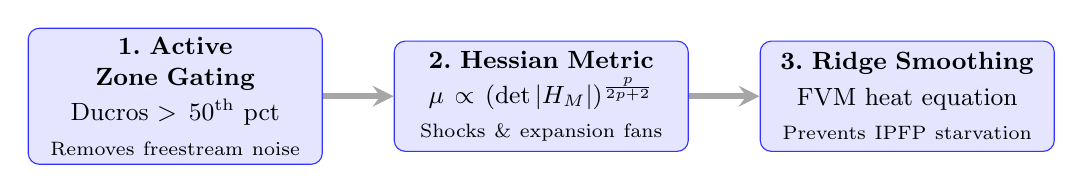
\begin{tikzpicture}[
    node distance=0.7cm and 0.9cm,
    block/.style={rectangle, draw=blue!80, fill=blue!10, text width=3.5cm,
                  text centered, rounded corners, minimum height=1.4cm, font=\small},
    arrow/.style={thick,->,>=stealth, draw=gray!70, line width=0.8mm}
]
    \node [block] (gate) {\textbf{1.\ Active Zone Gating}\\[0.2em]
                          Ducros $> 50^{\text{th}}$ pct\\[0.15em]
                          \scriptsize Removes freestream noise};
    \node [block, right=of gate] (hess) {\textbf{2.\ Hessian Metric}\\[0.2em]
                                          $\mu \propto (\det|H_M|)^{\frac{p}{2p+2}}$\\[0.15em]
                                          \scriptsize Shocks \& expansion fans};
    \node [block, right=of hess] (heat) {\textbf{3.\ Ridge Smoothing}\\[0.2em]
                                          FVM heat equation\\[0.15em]
                                          \scriptsize Prevents IPFP starvation};
    \draw [arrow] (gate) -- (hess);
    \draw [arrow] (hess) -- (heat);
\end{tikzpicture}
\end{center}

The Alauzet–Loseille metric density (two modes):
\[
    \texttt{det}:\quad \mu(x) \propto |\lambda_1\lambda_2|^{\frac{p}{2p+2}}, \qquad
    \texttt{eig}:\quad \mu(x) \propto |\lambda_{\max}|^{\frac{p}{2p+2}},
\]
where $\lambda_1,\lambda_2$ are eigenvalues of $|H_M|$, $p = 2$.

\end{frame}

\begin{frame}{Extracted Marginals — Diamond Body (M\,2.00 $\to$ M\,2.50)}

\begin{columns}
\begin{column}{0.5\textwidth}
\centering
\includegraphics[width=0.85\linewidth, height=0.72\textheight, keepaspectratio]%
    {Mach_interpolation/diamond/iso/hessian/det/drift_null/gmin0.005/Density_mu0.png}
{\small $\mu_0$ — Mach $2.00$ (\texttt{det} mode)}
\end{column}
\begin{column}{0.5\textwidth}
\centering
\includegraphics[width=0.85\linewidth, height=0.72\textheight, keepaspectratio]%
    {Mach_interpolation/diamond/iso/hessian/det/drift_null/gmin0.005/Density_mu1.png}\\[0.2em]
{\small $\mu_1$ — Mach $2.50$ (\texttt{det} mode)}
\end{column}
\end{columns}

\end{frame}

\begin{frame}{SB Density Transport — Diamond Body}

\centering
\includegraphics[width=0.65\linewidth, height=0.78\textheight, keepaspectratio]%
    {Mach_interpolation/diamond/iso/hessian/det/drift_null/gmin0.005/SB_Mach_density_density_transport.png}

\end{frame}

\begin{frame}{Drift Field $b_t = 2\gamma\nabla g_t$ — Diamond Body}

\centering
\includegraphics[width=0.65\linewidth, height=0.78\textheight, keepaspectratio]%
    {Mach_interpolation/diamond/iso/hessian/det/drift_null/gmin0.005/SB_Mach_drift_drift_field.png}

\end{frame}

\begin{frame}{Barycentric SB-CDI: IPFP Potentials $\to$ Mach Interpolation (1/2)}

\begin{block}{Step 1 — IPFP $\to$ Sinkhorn potentials $f, g$}
\[
    \mu_0 = e^f \cdot \mathcal{P}_1 e^g, \qquad \mu_1 = e^g \cdot \mathcal{P}_1 e^f.
\]
\end{block}

\begin{block}{Step 2 — Barycentric transport maps (boundary-corrected conditional means)}
Forward map $T$ (from $e^g$) and backward map $S$ (from $e^f$):
\[
    T(x) = \frac{\mathcal{P}_1[\,\mathrm{id}\cdot e^g\,](x)}{\mathcal{P}_1[\,e^g\,](x)} - \beta(x),
    \qquad
    S(x) = \frac{\mathcal{P}_1[\,\mathrm{id}\cdot e^f\,](x)}{\mathcal{P}_1[\,e^f\,](x)} - \beta(x),
\]
where $\beta(x) = \mathcal{P}_1[\mathrm{id}]/\mathcal{P}_1[1] - x$ removes the Neumann identity-leak.
\end{block}

\end{frame}

\begin{frame}{Barycentric SB-CDI: IPFP Potentials $\to$ Mach Interpolation (2/2)}

\begin{block}{Step 3 — Symmetric two-map CDI reconstruction (explicit, non-iterative)}
Sample each endpoint field along its own displaced pre-image, using the
forward map $T$ ($\mu_0\!\to\!\mu_1$) and backward map $S$ ($\mu_1\!\to\!\mu_0$):
\[
    W(t,x) = (1-t)\,x + t\,S(x), \qquad
    Z(t,x) = t\,x + (1-t)\,T(x),
\]
\[
    \hat{M}_t(x) = (1-t)\,M_0\!\bigl(W(t,x)\bigr) + t\,M_1\!\bigl(Z(t,x)\bigr).
\]
Gradient-free, no inversion, and exact at the endpoints:
$\hat{M}_0 = M_0$, $\hat{M}_1 = M_1$.
\end{block}

\end{frame}
\begin{frame}{Mach Interpolation — BaryCDI vs.\ HR Reference (\texttt{det} mode)}

\begin{columns}
\begin{column}{0.33\textwidth}
\centering
\includegraphics[width=\linewidth, height=0.36\textheight, keepaspectratio]%
    {Mach_interpolation/diamond/iso/hessian/det/drift_null/gmin0.005/Mach_BaryCDI_t0.20.png}\\[-0.1em]
{\scriptsize BaryCDI, $t=0.20$}\\[0.3em]
\includegraphics[width=\linewidth, height=0.36\textheight, keepaspectratio]%
    {../figures/diamond/h0.025/M_AOA0.00_M2.10_HLLC_MUSCL_SRK2_t4.00.png}\\[-0.1em]
{\scriptsize HR ref., $M=2.10$}
\end{column}
\begin{column}{0.33\textwidth}
\centering
\includegraphics[width=\linewidth, height=0.36\textheight, keepaspectratio]%
    {Mach_interpolation/diamond/iso/hessian/det/drift_null/gmin0.005/Mach_BaryCDI_t0.50.png}\\[-0.1em]
{\scriptsize BaryCDI, $t=0.50$}\\[0.3em]
\includegraphics[width=\linewidth, height=0.36\textheight, keepaspectratio]%
    {../figures/diamond/h0.025/M_AOA0.00_M2.25_HLLC_MUSCL_SRK2_t4.00.png}\\[-0.1em]
{\scriptsize HR ref., $M=2.25$}
\end{column}
\begin{column}{0.33\textwidth}
\centering
\includegraphics[width=\linewidth, height=0.36\textheight, keepaspectratio]%
    {Mach_interpolation/diamond/iso/hessian/det/drift_null/gmin0.005/Mach_BaryCDI_t0.80.png}\\[-0.1em]
{\scriptsize BaryCDI, $t=0.80$}\\[0.3em]
\includegraphics[width=\linewidth, height=0.36\textheight, keepaspectratio]%
    {../figures/diamond/h0.025/M_AOA0.00_M2.40_HLLC_MUSCL_SRK2_t4.00.png}\\[-0.1em]
{\scriptsize HR ref., $M=2.40$}
\end{column}
\end{columns}

\end{frame}

\begin{frame}{Mach Interpolation at $t = 0.5$ — \texttt{det} vs \texttt{eig} mode}

\begin{columns}
\begin{column}{0.5\textwidth}
\centering
\includegraphics[width=0.9\linewidth, height=0.66\textheight, keepaspectratio]%
    {Mach_interpolation/diamond/iso/hessian/det/drift_null/gmin0.005/Mach_BaryCDI_t0.50.png}\\[0.2em]
{\small Barycentric CDI (\texttt{det} mode)}
\end{column}
\begin{column}{0.5\textwidth}
\centering
\includegraphics[width=0.9\linewidth, height=0.66\textheight, keepaspectratio]%
    {Mach_interpolation/diamond/iso/hessian/eig/drift_null/gmin0.005/Mach_BaryCDI_t0.50.png}\\[0.2em]
{\small Barycentric CDI (\texttt{eig} mode)}
\end{column}
\end{columns}

\vspace{0.3em}
{\small\centering
On the diamond's straight oblique shocks, \texttt{det} gives the better, more
robust reconstruction; \texttt{eig} is preferred for curved shocks (e.g.\ the bump).\par}

\end{frame}

\begin{frame}{Quantitative Error: Wasserstein-2 Distance (1/2)}

\begin{block}{Kantorovich formulation}
Given interpolated field $\hat{M}_t$ and reference $M_t^{\mathrm{ref}}$, define
$\mu^M(x) \propto |M(x) - M_\infty|$ (normalized to unit mass on the mesh). The $W_2$ distance:
\[
    W_2^2(\mu, \nu) = \inf_{\pi\,\in\,\Pi(\mu,\nu)} \int_{\Omega\times\Omega} \|x - y\|^2\,d\pi(x, y).
\]
\end{block}

\begin{block}{Entropy-regularised OT cost}
With regularisation parameter $\varepsilon = 4\gamma_w$:
\[
    \mathrm{OT}_\varepsilon(\mu, \nu) = \min_{\pi\in\Pi(\mu,\nu)}
    \langle C,\pi\rangle - \varepsilon\,H(\pi),
    \quad C_{ij} = \|x_i - x_j\|^2.
\]
\end{block}

\end{frame}

\begin{frame}{Quantitative Error: Wasserstein-2 Distance (2/2)}

\begin{block}{Debiased Sinkhorn divergence}
Removes the entropic self-bias so that $S_\varepsilon(\mu,\mu) = 0$:
\[
    S_\varepsilon(\mu,\nu)
    = \mathrm{OT}_\varepsilon(\mu,\nu)
    - \tfrac{1}{2}\mathrm{OT}_\varepsilon(\mu,\mu)
    - \tfrac{1}{2}\mathrm{OT}_\varepsilon(\nu,\nu)
    \;\approx\; W_2^2(\mu,\nu).
\]
\end{block}

\begin{block}{Implementation via convolutional Sinkhorn (Solomon et al.\ 2015)}
The Gibbs kernel $K_{ij} = e^{-\|x_i-x_j\|^2/\varepsilon}$ is approximated by the FVM heat
semigroup $e^{\gamma_w\Delta}$, \emph{the same operator used inside IPFP}.

Dual value at convergence: $\mathrm{OT}_\varepsilon = \varepsilon\!\bigl(\langle F, \mu\rangle + \langle G, \nu\rangle\bigr)$,
with Sinkhorn potentials $F$, $G$ satisfying
\[
    G = \log\nu - \log\mathcal{P}_1\!\bigl[e^{F}\bigr], \quad
    F = \log\mu - \log\mathcal{P}_1\!\bigl[e^{G}\bigr], \quad
    W_2 \approx \sqrt{\max(S_\varepsilon, 0)}.
\]
Parameters: $\gamma_w = 0.005$\;($\sigma_w \approx 0.10$), 50 Sinkhorn iterations.
\end{block}

\end{frame}

\begin{frame}{Error vs.\ High-Resolution Reference — Diamond (\texttt{det} mode)}

\begin{columns}
\begin{column}{0.5\textwidth}
\centering
\includegraphics[width=\linewidth, height=0.72\textheight, keepaspectratio]%
    {Mach_interpolation/diamond/iso/hessian/det/drift_null/gmin0.005/Mach_L2_Linf_l2_linf_errors.png}\\[0.2em]
{\small $L_2$ and $L_\infty$ Mach errors vs.\ 9 references}
\end{column}
\begin{column}{0.5\textwidth}
\centering
\includegraphics[width=\linewidth, height=0.72\textheight, keepaspectratio]%
    {Mach_interpolation/diamond/iso/hessian/det/drift_null/gmin0.005/Mach_Wasserstein.png}\\[0.2em]
{\small $W_2$ distance on $|M - M_\infty|$ density}
\end{column}
\end{columns}

\end{frame}

\begin{frame}{Absolute Error Heatmaps — Diamond (\texttt{det} mode)}

\begin{columns}
\begin{column}{0.5\textwidth}
\centering
\includegraphics[width=0.9\linewidth, height=0.72\textheight, keepaspectratio]%
    {Mach_interpolation/diamond/iso/hessian/det/drift_null/gmin0.005/AbsErr_Linear_abs_error.png}\\[0.2em]
{\small Linear interpolation}
\end{column}
\begin{column}{0.5\textwidth}
\centering
\includegraphics[width=0.9\linewidth, height=0.72\textheight, keepaspectratio]%
    {Mach_interpolation/diamond/iso/hessian/det/drift_null/gmin0.005/AbsErr_BaryCDI_abs_error.png}\\[0.2em]
{\small Barycentric CDI (\texttt{det})}
\end{column}
\end{columns}

\end{frame}


\begin{frame}{Schrödinger Bridge with a Reference Drift}

\begin{block}{Reference SDE and Girsanov energy}
\[
    dX_t = \bt_t(X_t)\,dt + \sqrt{2\gamma}\,dW_t,
    \qquad
    \mathcal{J}(\rho,b) = \int_0^1\!\!\int_{\mathbb{R}^d}
        \tfrac{1}{2}\,\|b_t - \bt_t\|^2\,\rho_t\,dx\,dt.
\]
\end{block}

\begin{block}{Optimal control and advected HJB equation}
\[
    b_t = \bt_t + \nabla\phi_t,
    \qquad
    \partial_t\phi_t + \tfrac{1}{2}\|\nabla\phi_t\|^2
        + \bt_t\cdot\nabla\phi_t + \gamma\,\Delta\phi_t = 0.
\]
\end{block}

\medskip
$\bt$ pre-transports the shocks $M_0\!\to\!M_1$; the bridge only corrects the
residual $\nabla\phi_t$ — small correction $\Rightarrow$ well-conditioned at small $\gamma$.

\end{frame}

\begin{frame}{Hopf–Cole: Two Transport–Diffusion Equations}

With $\rho_t = \eta_t\,\eta^*_t$, the drifted HJB linearizes to advected heat equations:

\begin{block}{Backward — generator $\mathcal{L} = \bt\cdot\nabla + \gamma\Delta$ (non-conservative)}
\[
    \partial_t \eta^*_t + \bt_t\cdot\nabla\eta^*_t + \gamma\,\Delta\eta^*_t = 0.
\]
\end{block}

\begin{block}{Forward — adjoint $\mathcal{L}^*$ (conservative)}
\[
    \partial_t \eta_t + \nabla\!\cdot(\bt_t\,\eta_t) - \gamma\,\Delta\eta_t = 0,
    \qquad
    \nabla\!\cdot(\bt\,\eta) = \bt\cdot\nabla\eta + (\nabla\!\cdot\bt)\,\eta.
\]
\end{block}

\medskip
The drift breaks self-adjointness: two distinct operators, differing by the
reaction term $(\nabla\!\cdot\bt)\,\eta$ — kept, since the windowed $\bt$ has
$\nabla\!\cdot\bt \neq 0$.  $\bt\equiv0$ recovers the two heat equations.

\end{frame}

\begin{frame}{IPFP with a Reference Drift}

$\mathcal{Q}_\tau = e^{\tau\mathcal{L}}$: transition operator of the drifted SDE;
\quad $\mathcal{Q}^{\dagger}_\tau = e^{\tau\mathcal{L}^*}$: its adjoint.

\begin{block}{Drifted IPFP iterations}
\[
    f^{(k+1)} = \log\mu - \log\mathcal{Q}_1\!\bigl[e^{g^{(k)}}\bigr],
    \qquad
    g^{(k+1)} = \log\nu - \log\mathcal{Q}^{\dagger}_1\!\bigl[e^{f^{(k+1)}}\bigr].
\]
\end{block}

\begin{itemize}
    \item $\mathcal{Q}^{\dagger}_1$: TPFA diffusion $+$ conservative first-order upwind advection.
    \item $\mathcal{Q}_1$: \emph{exact area-weighted transpose} of $\mathcal{Q}^{\dagger}_1$
          $\Rightarrow$ M-matrix (positivity at any Péclet),
          $\langle\mathcal{Q}u,v\rangle = \langle u,\mathcal{Q}^{\dagger}v\rangle$ to machine precision.
    \item $\bt\equiv0 \;\Rightarrow\; \mathcal{Q}_1=\mathcal{Q}_1^{\dagger}=\mathcal{P}_1$:
          exact reduction to the driftless IPFP.
\end{itemize}

\end{frame}

\begin{frame}{Analytic Drift for the Diamond Airfoil (1/2) — Wave Angles}

The LE and TE shocks rotate between their $M_0$ and $M_1$ wave angles:

\begin{block}{$\theta$–$\beta$–$M$ relation (weak root) — LE family}
\[
    \tan\theta = 2\cot\beta_s\,\frac{M^2\sin^2\beta_s - 1}{M^2(\gamma_g+\cos2\beta_s)+2},
    \qquad
    \beta_s^{\mathrm{LE}}(M) = \beta_s(\alpha, M).
\]
\end{block}

\begin{block}{TE family — LE shock $\to$ Prandtl–Meyer($2\alpha$) $\to$ TE shock}
\[
    \nu(M_b) = \nu(M_a) + 2\alpha,
    \qquad
    \beta_s^{\mathrm{TE}}(M) = \beta_s(\alpha, M_b(M)).
\]
\end{block}

\begin{block}{Ray angles and rotation rates,\; $M(t)=(1-t)M_0+tM_1$}
\[
    \psi_{\mathrm{LE}} = \beta_s^{\mathrm{LE}}, \qquad
    \psi_{\mathrm{TE}} = \beta_s^{\mathrm{TE}}-\alpha, \qquad
    \omega_\kappa(t) = \tfrac{d\beta_s^{\kappa}}{dM}\big|_{M(t)}\,(M_1-M_0).
\]
\end{block}

\end{frame}

\begin{frame}{Analytic Drift for the Diamond Airfoil (2/2) — Windowed Rotation}

\begin{block}{Four windowed rigid rotations about the apexes $\av_\kappa$}
\[
    \boxed{\;
    \bt(t,x) = \sum_{\kappa\in\{\mathrm{LE},\mathrm{TE}\}}\sum_{\sigma=\pm1}
        \sigma\,\omega_\kappa(t)\,w_{\kappa,\sigma}(t,x)\,\R\,(x-\av_\kappa),
    \qquad
    \R = \bigl(\begin{smallmatrix}0&-1\\1&0\end{smallmatrix}\bigr)
    \;}
\]
\[
    w_{\kappa,\sigma} = e^{-\mathrm{dist}_{\kappa,\sigma}^2/\sigma_w(s)^2}\,
        \mathbf{1}[s_{\kappa,\sigma}>0],
    \qquad
    s_{\kappa,\sigma} = (x-\av_\kappa)\cdot\dhat_{\kappa,\sigma}.
\]
\end{block}

Zero in the freestream; the conical band $\sigma_w(s)$ covers the swept wedge;
$\nabla\!\cdot\bt\neq0$ $\Rightarrow$ enters through the conservative $\mathcal{Q}^{\dagger}$.

\medskip
\centering
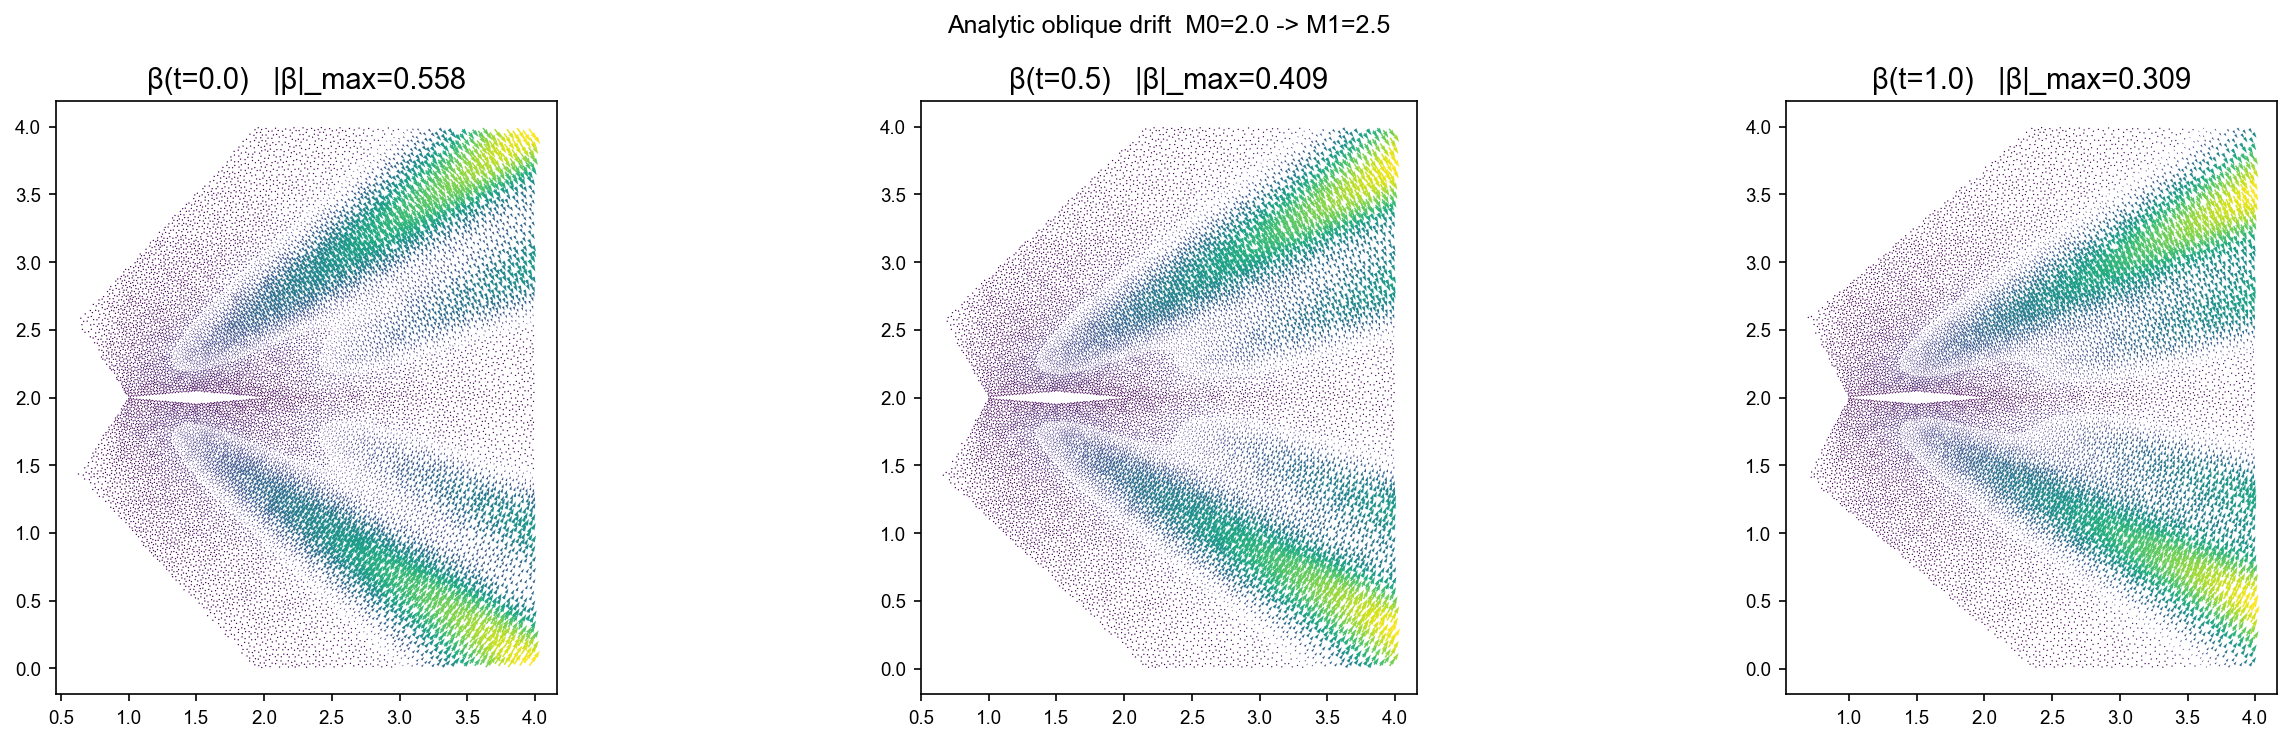
\includegraphics[width=0.7\linewidth, keepaspectratio]{drift_beta_quiver.png}

\end{frame}

\begin{frame}{Drifted vs.\ Driftless Bridge — Error vs.\ HR Reference (\texttt{det} mode)}

\begin{columns}
\begin{column}{0.5\textwidth}
\centering
\includegraphics[width=\linewidth, height=0.72\textheight, keepaspectratio]%
    {Mach_interpolation/diamond/iso/hessian/det/drift_null/gmin0.005/Mach_L2_Linf_l2_linf_errors.png}\\[0.2em]
{\small No drift, $\gamma_{\mathrm{sb}}=0.005$}
\end{column}
\begin{column}{0.5\textwidth}
\centering
\includegraphics[width=\linewidth, height=0.72\textheight, keepaspectratio]%
    {Mach_interpolation/diamond/iso/hessian/det/drift_oblique/gmin0.0001/Mach_L2_Linf_l2_linf_errors.png}\\[0.2em]
{\small Oblique drift, $\gamma_{\mathrm{sb}}=0.001$}
\end{column}
\end{columns}

\vspace{0.3em}
{\small\centering The drift lets IPFP run stably at a $5\times$ smaller
$\gamma_{\mathrm{sb}}$ — smaller entropic blur, sharper reconstructed shocks.\par}

\end{frame}

\begin{frame}{Drifted Bridge — Density Transport and Drift Field (\texttt{det} mode)}

\begin{columns}
\begin{column}{0.5\textwidth}
\centering
\includegraphics[width=0.9\linewidth, height=0.72\textheight, keepaspectratio]%
    {Mach_interpolation/diamond/iso/hessian/det/drift_oblique/gmin0.0001/SB_Mach_density_density_transport.png}\\[0.2em]
{\small Density transport under $\mathcal{Q},\mathcal{Q}^\dagger$}
\end{column}
\begin{column}{0.5\textwidth}
\centering
\includegraphics[width=0.9\linewidth, height=0.72\textheight, keepaspectratio]%
    {Mach_interpolation/diamond/iso/hessian/det/drift_oblique/gmin0.0001/SB_Mach_drift_drift_field.png}\\[0.2em]
{\small Drift field $b_t = \bt_t + 2\gamma\nabla g_t$ at $t=0.5$}
\end{column}
\end{columns}

\end{frame}

\begin{frame}{Mach Interpolation with Oblique Drift — \texttt{det} vs \texttt{eig} ($t=0.5$)}

\begin{columns}
\begin{column}{0.5\textwidth}
\centering
\includegraphics[width=0.9\linewidth, height=0.66\textheight, keepaspectratio]%
    {Mach_interpolation/diamond/iso/hessian/det/drift_oblique/gmin0.0001/Mach_BaryCDI_t0.50.png}\\[0.2em]
{\small Barycentric CDI, oblique drift (\texttt{det})}
\end{column}
\begin{column}{0.5\textwidth}
\centering
\includegraphics[width=0.9\linewidth, height=0.66\textheight, keepaspectratio]%
    {Mach_interpolation/diamond/iso/hessian/eig/drift_oblique/gmin0.0001/Mach_BaryCDI_t0.50.png}\\[0.2em]
{\small Barycentric CDI, oblique drift (\texttt{eig})}
\end{column}
\end{columns}

\vspace{0.3em}
{\small\centering Both hessian modes remain stable at $\gamma_{\mathrm{sb}}=0.001$
once the drift pre-transports the shock rays.\par}

\end{frame}

\begin{frame}{Absolute Error Heatmaps — Oblique Drift (\texttt{det} mode, $\gamma_{\mathrm{sb}}=0.001$)}

\begin{columns}
\begin{column}{0.5\textwidth}
\centering
\includegraphics[width=0.9\linewidth, height=0.72\textheight, keepaspectratio]%
    {Mach_interpolation/diamond/iso/hessian/det/drift_oblique/gmin0.0001/AbsErr_Linear_abs_error.png}\\[0.2em]
{\small Linear interpolation}
\end{column}
\begin{column}{0.5\textwidth}
\centering
\includegraphics[width=0.9\linewidth, height=0.72\textheight, keepaspectratio]%
    {Mach_interpolation/diamond/iso/hessian/det/drift_oblique/gmin0.0001/AbsErr_BaryCDI_abs_error.png}\\[0.2em]
{\small Barycentric CDI (oblique drift)}
\end{column}
\end{columns}

\end{frame}

\end{document}